\chapter{Haskell}
\label{haskell}

Haskell is a functional language developed in the 1990s. Designed to be lazy, pure and to support type classes \cite{hudak2007history}, the language has been evolving since its creation. This chapter will provide examples of some of the functional programming concepts introduced in Chapter \ref{fp} using the Haskell language. This chapter is not a "Haskell Tutorial"; its primary goal is to present the concepts of functional programming that will be used in the practical section and, therefore, will be one of the central objects of study of this work. The fundamental ideas of the next section come from \cite{hutton2016programming}, and from \cite{fp101em} (course at TU Delft); those are also good references to get started into Haskell programming.

The development of the Haskell language started in 1987 \cite{hudak2007history}, but its foundations started a few decades before, with Alonzo's Church Lambda Calculus. In the 1970s, John Backus inaugurated the term \textit{Functional style} in his work \cite{backus1978can}, motivating a meeting of programming language researches ten years later. This group officially started the works on the Haskell language.

The principal features of the Haskell language \cite{hutton2016programming} are listed below:

\begin{itemize}\label{lsthbenefits}
\item Concise programs - Haskell's syntax is designed to be compressed and to have just a few keywords. \textit{List Comprehensions}, for example, are a concise way to navigate on a list, create new ones, filter elements or transform the existing ones. No need for explicit loops (like \lstinline!while!) or nested if/else blocks.
\item Type system - Haskell's type system helps programmers to detect incompatibility errors at compile time (the functions often require the expected input and output types). Haskell supports polymorphism and overloading, providing the developers with a wide range of features.
\item Recursive functions - One and probably the most important way to navigate through a collection of elements is using \textbf{recursion}. To determine when to stop or to continue, recursion can be combined with \textbf{pattern matching}.
\item Higher-order functions - Functions can receive other functions as arguments, as well as return them as values. A \textbf{higher order function} abstracts the behaviour of a group of functions, wrapping it up in another function.
\item Effectful functions - A function is called \textbf{pure} when it produces the same output given the same inputs, without any interference. In some circumstances, there may be \textit{side effects}, causing unexpected outputs. Operations that involve files are a good example of impurity. If a function requires a file, it may or may not be present, causing the function to have multiple outputs for the same inputs. It will be an \textbf{impure} function. Haskell provides mechanisms to deal with this impurity scenario: \textit{monads} and \textit{applicatives}.
\item Lazy evaluation - In Haskell, a computation is not performed until it is required by another function. This mechanism avoids unnecessary computations and allows the usage of infinite structures, such as infinite lists.
\item Equational reasoning - Combined with induction, it can be used to transform, execute and demonstrate properties of Haskell programs.
\end{itemize}


\section{Function and Types in Haskell}

Recall that one of the aspects of functional programming is having a style closer to a mathematical representation. In this context, \lstinline[language=haskell]{f x} in the Haskell language corresponds to the mathematical function application $ f(x) $. In other words, an empty, blank space represents a function application.

\subsection{Basic types}

Another topic that arises in functional languages are \textbf{types}: they are a collection of related values, as seen in \cref{lst:typesdecla}.

\begin{lstlisting}[language=Haskell, label={lst:typesdecla}, caption={Types for variables and expressions}, captionpos=b]
v::T -- v has type T
e::T -- The evaluation of the expression e will produce a value of type T
\end{lstlisting}

In Haskell, every expression must have a type. For this language, it is possible to either manually define the types or to have them inferred using the \textbf{type inference} process. This step happens before the proper evaluation, so if there is anything that does not match the possible type (for example, adding a string with an integer), the code will not compile. Making types explicit when writing functions is a good practice in Haskell. Mathematically speaking, this is shown in \cref{fig:proof1}:

\begin{figure}[H]
\caption{Transient Analysis - Example Circuit}
\label{fig:proof1}
\begin{prooftree}
  \AxiomC{$f::A \rightarrow B $}
  \AxiomC{$ e::A $}
  \BinaryInfC{$ f e::B $}
\end{prooftree}
\end{figure}

Figure \ref{fig:proof1} states that if there is a function \textbf{f} that maps an argument of type \textbf{A} to a result of type \textbf{B} and \textbf{e} is an expression of type \textbf{A}, the application of the function \textbf{f} will have the type \textbf{B}.

Haskell programs are labelled as \textit{type safe} because the compiler guarantees the absence of type errors during run time. One downside about this feature is that sometimes a valid expression may be misinterpreted during the type inference process, causing it to reject a correct expression.

Some examples of built-in types in Haskell are Int, Float, Double. There are also more sophisticated built-in types in Haskell - Lists, collections of elements of the same types; and Tuples, finite sequences of components, which can be of different types. An example can be found in \cref{lst:examplesbuiltintypes}.

\begin{lstlisting}[language=Haskell, label={lst:examplesbuiltintypes}, caption={Lists and Tuples}, captionpos=b]
[1,2,3] -- A List of Integers
("Hanneli","UNIFEI",2019,True) -- A Tuple of arity four (four elements)
\end{lstlisting}

Conceptually, Lists require a specification of the type they will convey. It is reasonable to have lists of Integers, Floats and Strings, for examples. Generalising, there is the type \lstinline[language=haskell]{List a}, where \textbf{a} is a variable to indicate a type. A type (in this case, \textbf{List}) that contains one or more type variables (in this case, \textbf{a}), is a \textbf{polymorphic type}.


A \textbf{List} like [1,2,3] is equivalent to \lstinline[language=haskell]{(1:(2:(3:[])))}. From this alternative representation it is possible to see that lists are recursively compounded. Initially, there is the empty list \lstinline[language=haskell]{[]}, and then 3, then 2, then 1 are appended. In functional languages, recursion is very important to compose several data structures. Recursion is also the basic looping mechanism. In Java or C++, it is common to find a \textbf{for} loop accessing items of collections by indexes. In contrast, Haskell relies on recursion to perform operations across lists. For example, multiplication can be defined as a recursive sum as shown in \cref{lst:recursivesumexample}.


\begin{lstlisting}[language=Haskell, label={lst:recursivesumexample}, caption={Recursion}, captionpos=b]
mult _ 0 = 0 -- Base case
mult n m = (mult n (m - 1)) + n -- Recursive call
\end{lstlisting}


Given that a function can receive other functions as arguments and return other functions, a function is itself a type. That means functions receiving multiple parameters can be rewritten as functions that receive a single parameter and return another function. This is called \textbf{currying}. For example, when declaring a function \lstinline!adds! to add two integers, the function type can be defined as something that receives two integers and returns another integer ( \lstinline!adds :: Int -> Int -> Int! ) or as a function that takes only one integer and returns another function that takes the second integer and returns the result: \lstinline!adds :: Int -> (Int -> Int)!. In the previous example, the parentheses are optional, since the \lstinline!->! (named 'arrow function') is interpreted as right-associative. So \lstinline!Int -> Int -> Int -> Int! is the same as \lstinline!Int -> (Int -> (Int -> Int))!.

However, function application (denoted by a simple space character \lstinline!" "!) associates to the left. So \lstinline!adds x y z! means \lstinline!((adds x) y) z!.

In Haskell, the concept of \textit{class} differs from the idea of the object-oriented languages. A class is a collection of types that supports overloaded operations (\textit{methods}). For example, \textit{Equality} is a class that contains a method \lstinline!(==)! under the type signature of \lstinline!(==) :: a -> a -> Bool!, that determines if an element of the collection of types \lstinline!a! is equal to another of the same type, a Bool result must be returned. Ordering (\lstinline!ord!), \lstinline!Show!, \lstinline!Read!, Numerical (\lstinline!Num!) and \lstinline!Fractional! are other examples of Haskell classes.


\subsection{Function structure and resources}\label{haskell:fnstr}

Haskell supports \lstinline!if/else! blocks (example: \lstinline!if n == 0 then 0 else 1!), but it is much more common to use \textit{guard} expressions (see \cref{lst:letexprsimplified1}) or \textit{pattern matching} (see \cref{lst:pmcase}):

\begin{lstlisting}[language=Haskell, numbers=left, caption={Pattern matching with case}, captionpos=b, label={lst:pmcase}]
condutance :: ComponentData -> Double -> Double
condutance component dt =
  case componentType component of
    Resistor -> 1.0 / (magnitude component)
    Capacitor -> (magnitude component) * 0.000001 * 2 / dt
    Inductor -> dt / (2 * 0.001 * (magnitude component))
    _ -> 0.0
\end{lstlisting}

It is possible to pattern match against Lists, Tuples and other types.

It is feasible to define auxiliary, nameless functions. They are called \textbf{lambda} expressions and a similar concept is present in some object-oriented languages such as Python. In \cref{lst:lambdafunction}, there is a lambda expression right after \lstinline!map!. This anonymous function specifies one should be added to the value of each component of a collection. \lstinline!\! indicates the declaration of a lambda expression. The name 'lambda' expression originates from $\lambda$-Calculus (visit \cref{sec:lc} for more information).

\begin{lstlisting}[language=Haskell, numbers=left, caption={Lambda functions}, captionpos=b, label={lst:lambdafunction}]
map (\r -> (r + 1)) [1, 2, 3]
\end{lstlisting}

\lstinline!map! applies another function to each element of a list. For example, to add 2 to all the elements of \lstinline![1, 2, 3]!, one can invoke the \lstinline!map! function as in \lstinline!map (+2) [1, 2, 3]!. 

\subsection{Higher order functions}

Higher-order functions allow common programming patterns to be wrapped in a function. To build the intuition on this topic, it is reasonable to sketch an example with the \lstinline!fold! function. "Folding" a list means to compress it following a certain operation. For example, \lstinline!foldl (+) 0 [1, 2, 3]! returns 6; the 0 is the initial buffer. $+$ is the operation, and $0 + 1 + 2 +3$ is the result of \lstinline!fold!. Alternatively, \lstinline!foldl (+) 1 [1, 2, 3]! returns 7, because the initial accumulator is 1.

"\lstinline!fold! takes an 'initial answer' \lstinline!acc! and uses [a function] \lstinline!f! to 'combine' \lstinline!acc! and the first element of the list, using this as the new 'initial answer' for 'folding' over the rest of the list"\cite{plcoursera}. A collection can be folded to the left with \lstinline!foldl! or to the right with \lstinline!foldr!. The \cref{lst:foldl} describes the implementation of a left fold, named as \lstinline!foldl2!, since \lstinline!foldl! is the name of the funciton in the standard implementation of the Haskell language.

\begin{lstlisting}[language=Haskell, numbers=left, caption={fold left}, captionpos=b, label={lst:foldl}]
foldl2 f v [] = v
foldl2 f v (x:xs) = foldl2 f (f v x) xs
\end{lstlisting}

The type signature of \lstinline!foldl! is given by \cref{lst:foldltypesig}:

\begin{lstlisting}[language=Haskell, numbers=left, caption={fold left type signature}, captionpos=b, label={lst:foldltypesig}]
foldl :: (a -> b -> a) -> a -> [b] -> a
\end{lstlisting}

Functions can be composed the same way they are composed in mathematics. The higher-order composition function (denoted by the operator \lstinline! . !) allows the function composition $ f \circ g $ with the syntax \lstinline!f . g! .

\subsection{Composite types}

It is possible to define custom types in Haskell by using the keyword \textbf{data}. The \cref{lst:haskellex1ch4} is an example of a new data called Shape, which has two possible constructions: it can be a Circle or a Rectangle.

\begin{lstlisting}[language=Haskell, label=getinfo, caption={Custom types}, captionpos=b, label={lst:haskellex1ch4}]
data Shape = Circle Float | Rectangle Float Float

square::Float -> Shape
square n = Rectangle n n 

\end{lstlisting} 

\textbf{Rectangle} and \textbf{Circle} are constructor functions. They exist for building pieces of data, but they do not carry the defining equations. The logic to build the actual rectangle is in the function \textbf{square}. This is consistent with the principles of functional programming: the data is isolated, and the basic method of computation to build anything is the application of functions.

The keyword \textit{type} adds an alias to existing types. For example, \lstinline!type String = [Char]!, implies that \lstinline!String! is just a List of \lstinline!Char!. Type declarations can be parameterised by other types. For example, \lstinline!type Pair a = (a, a)!.

\section{Impure functions}
\label{sideeffects}

One of the key ideas in functional programming is the concept of \textit{pure functions}. They have no side effects (they do not mutate any state of the program or change non-local variables). These functions also return the same value given the same input arguments, just as a regular mathematical function.

However, I/O operations can have side effects. For example, opening a file may succeed or may throw an error, either because the file does not exist or because it is corrupted. Note that this problem has nothing to do with manipulating the information on a file; it is an external problem. Realistically, it is only possible to have a code that expects the possibility of a side effect. Languages like Java deal with this scenario by throwing run time exceptions. 

Haskell represents impurity with the \lstinline!IO! type. Expressions of this type are named as \textit{actions}. 

The use case presented in this work requires, from the very first beginning, an action that will generate side effects - reading CSV files with the input data. A function to read and parse the data can have side effects when (a) the file is not in the specified directory; (b) the file does not exist; (c) the file is empty; (d) the file is corrupted. The type of a parsing function must incorporate the possibility of these side effects, and for that matter, two elements are required:
\begin{enumerate}
  \item an action to change the context from pure to impure (\lstinline!return! function in \cref{lst:donotation});
  \item a sequencing operator to apply the parser and call the result, then reapply the parser, get the result and repeat the process until the end of the file is reached. A sequence of actions can be chained with the \lstinline!do! notation as seen in \cref{lst:donotation}.
\end{enumerate}


\begin{lstlisting}[language=Haskell, caption={do notation; Note: this is just a didactic draft example.}, captionpos=b, label={lst:donotation}]
do
  eitherSimulation <- decodeSimulationFromFile "data/simulation.csv"
  componentsList <- decodeItemsFromFile "data/components.csv"
  return (eitherSimulation, componentList)
\end{lstlisting}


\section{Monads}
\label{hsmonads}

Haskell supports even more generic sets of functions - some of them can be generalised over a range of parameterised types (lists, trees, IO). For example, it is possible to generalise the idea of \lstinline!map! to other structures rather than Lists. In the reference implementation of this work, in many scenarios \lstinline!map! occurs in a \lstinline!Vector!. This generalisation is seen on \cref{lst:mapvecfnd}:

\begin{lstlisting}[language=Haskell, numbers=left, caption={map in a Vector}, captionpos=b, label={lst:mapvecfnd}]
gkm :: Vector ComponentData -> Double -> Vector Double
gkm components dt =
  Vector.map (\c -> condutance c dt) components
\end{lstlisting}

There is a class of types supporting the \lstinline!map! function - this is the \lstinline!Functor! class, with \lstinline!fmap! as the generic function that maps another function over each element of a structure \cite{hutton2016programming}.

\begin{lstlisting}[language=Haskell, numbers=left, caption={Functor class}, captionpos=b, label={lst:functorfmap}]
class Functor f where
  fmap :: (a -> b) -> f a -> f b
\end{lstlisting}

\ref{lst:mapvecfnd} is an example of a Functor. Functors work for single-element functions. It is possible to generalise the idea of Functor itself, making it support any number of parameters, as suggested in \cref{genfunctors}.

\begin{figure}[H]
   \centering
   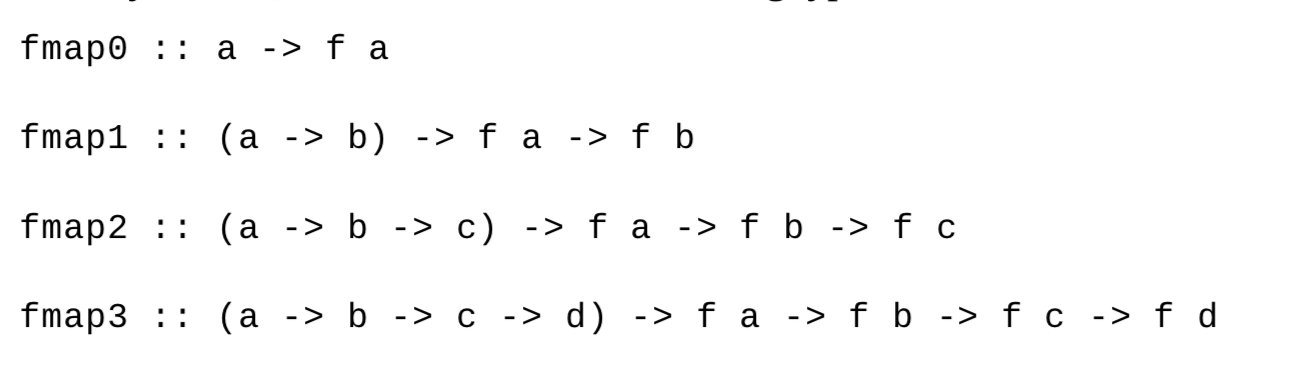
\includegraphics[width=0.9\textwidth]{img/functorapplicative.png}
   \caption{Generalising functors}
   \label{genfunctors}
\end{figure}
\cite{hutton2016programming}

Two basic functions are capable of encoding the desired generalisation. They are built using the idea of currying and are described in  \cref{lst:applicatives}:


\begin{lstlisting}[language=Haskell, numbers=left, caption={Applicatives}, captionpos=b, label={lst:applicatives}]
class Functor f=> Applicative f where
  pure :: a -> f a
  (<*>) :: f (a -> b) -> f a -> f b 
\end{lstlisting}

This pair of functions is called \textbf{Applicative Functor} (or simply \textbf{Applicatives}). Examples of its usage can also be found in the implementation of Haskell ETR-P in \cref{lst:usingapplicatives}:

\begin{lstlisting}[language=Haskell, numbers=left, caption={Using Applicatives}, captionpos=b, label={lst:usingapplicatives}]
instance FromNamedRecord ComponentData where
  parseNamedRecord m =
    ComponentData
      <$> m .: "Element Type"
      <*> m .: "Node K"
      <*> m .: "Node M"
      <*> m .: "Value"
      <*> m .: "Source param 1"
      <*> m .: "Source param 2"
      <*> m .: "Plot"

instance FromField ComponentType where
  parseField "R" =
    pure Resistor

  parseField "L" =
    pure Inductor

  parseField "C" =
    pure Capacitor

  parseField "EDC" =
    pure EDC

  parseField "EAC" =
    pure EAC

  parseField otherType =
    Other <$> parseField otherType
\end{lstlisting}


In Haskell, it is possible to encode a possibility of failure in the function's type. The \lstinline!Maybe! type wraps a success branch (named \lstinline!Just a!) or a possible failure, represented by the absence of value (represented by \lstinline!Nothing!). The \textbf{bind} operator \lstinline!>>=! takes an argument of type "a"  and a function of type \lstinline!a -> b!. Both can fail, the argument and the function. \lstinline!>>=! returns a result of type "b", which can also be a failure (encoded as a Maybe) as shown in \cref{lst:bindoperator}:


\begin{lstlisting}[language=Haskell, numbers=left, caption={The bind operator}, captionpos=b, label={lst:bindoperator}]
(>>=) :: Maybe a -> (a -> Maybe b) -> Maybe b
mx >>= f = case mx of
           Nothing -> Nothing
           Just x -> f x
\end{lstlisting}

It is also necessary to have a function that provides a connection between pure functions and actions (impure). This is the \textbf{return} function, with the signature defined in \cref{lst:returnfunc}.

\begin{lstlisting}[language=Haskell, numbers=left, caption={The return}, captionpos=b, label={lst:returnfunc}]
return :: a -> IO a
\end{lstlisting}

The \lstinline!return! function defined in \cref{lst:returnfunc} has nothing to do with the "return" statements found in languages like C.

A \textbf{Monad} arises from the combination of these two elements, \lstinline!>>=! and \lstinline!return!. A Monad is an applicative that supports both of these operations. "Every Monad is an applicative functor"\cite{lipovaca2011learn} in its generalised form, as proposed in \ref{genfunctors}. This work will not explore in detail the powerful constructions built on the monadic style. A complete example of Monad applications can be found on the work of \cite{hutton1998monadic}. The code in \cref{lst:parserex} and \cref{lst:parserexmonad} describe a Monadic parser with the two principal elements of a Monad: the \lstinline!return! and bind operator \lstinline!>>= !:

\begin{lstlisting}[language=Haskell, caption={Declaring the type Parser}, captionpos=b, label={lst:parserex}]
newtype Parser a = Parser (String -> [(a,String)])
\end{lstlisting}

\begin{lstlisting}[language=Haskell, caption={Declaring the type Parser}, captionpos=b, label={lst:parserexmonad}]
instance Monad Parser where
  return a = Parser (\cs -> [(a,cs)])
  p >>= f = Parser (\cs -> concat [parse (f a) cs' |
    (a,cs') <- parse p cs])
\end{lstlisting}

\section{Advanced Features and fields of study}

The previous sections provided the basic concepts required to understand and interpret the code in Chapter \ref{implhs}. However, the Haskell language has been evolving continuously and it has advanced topics which are also out of the scope of this work. Just to give a taste to the reader, some of the active research topics involve (but are not limited to): Deep EDSL \cite{gill2014domain}, verification of Haskell programs with type theory \cite{abel2005verifying}, constraint solving \cite{hallahan2019g2q}, Monad transformers \cite{schrijvers2016monad}, verification of Haskell programs in proof interactive theorem provers (like Coq \cite{coqurl} or Liquid Haskell \cite{liquidhaskell}, see \cite{Christiansen} and \cite{vazou2016liquid}), program synthesis in Haskell \cite{Finkbeiner}, etc.










